\chapter{Design: How David and I applied these tools to make the REIXS optical design}

\section{Application to spectrometer design}
\subsection{Design Goals: (simultaneously)}
          - Highest resolution: "Resolution, �Eres, is a measure of smallest amount by which two energies can differ and still be distinguished (or re- solved) by a given spectrometer."
          - Fast experiments (high efficiency)
          - Reference: Stated goals from David's thesis
\subsection{Comparative examples}
          - High-res beamline at SLS; 
          - BL8 (workhorse); 
          - commercial XES350
          
FIGURE 4a: comparison of resolution, REF david's thesis

\begin{figure}[htbp] %  figure placement: here, top, bottom, or page
   \centering
   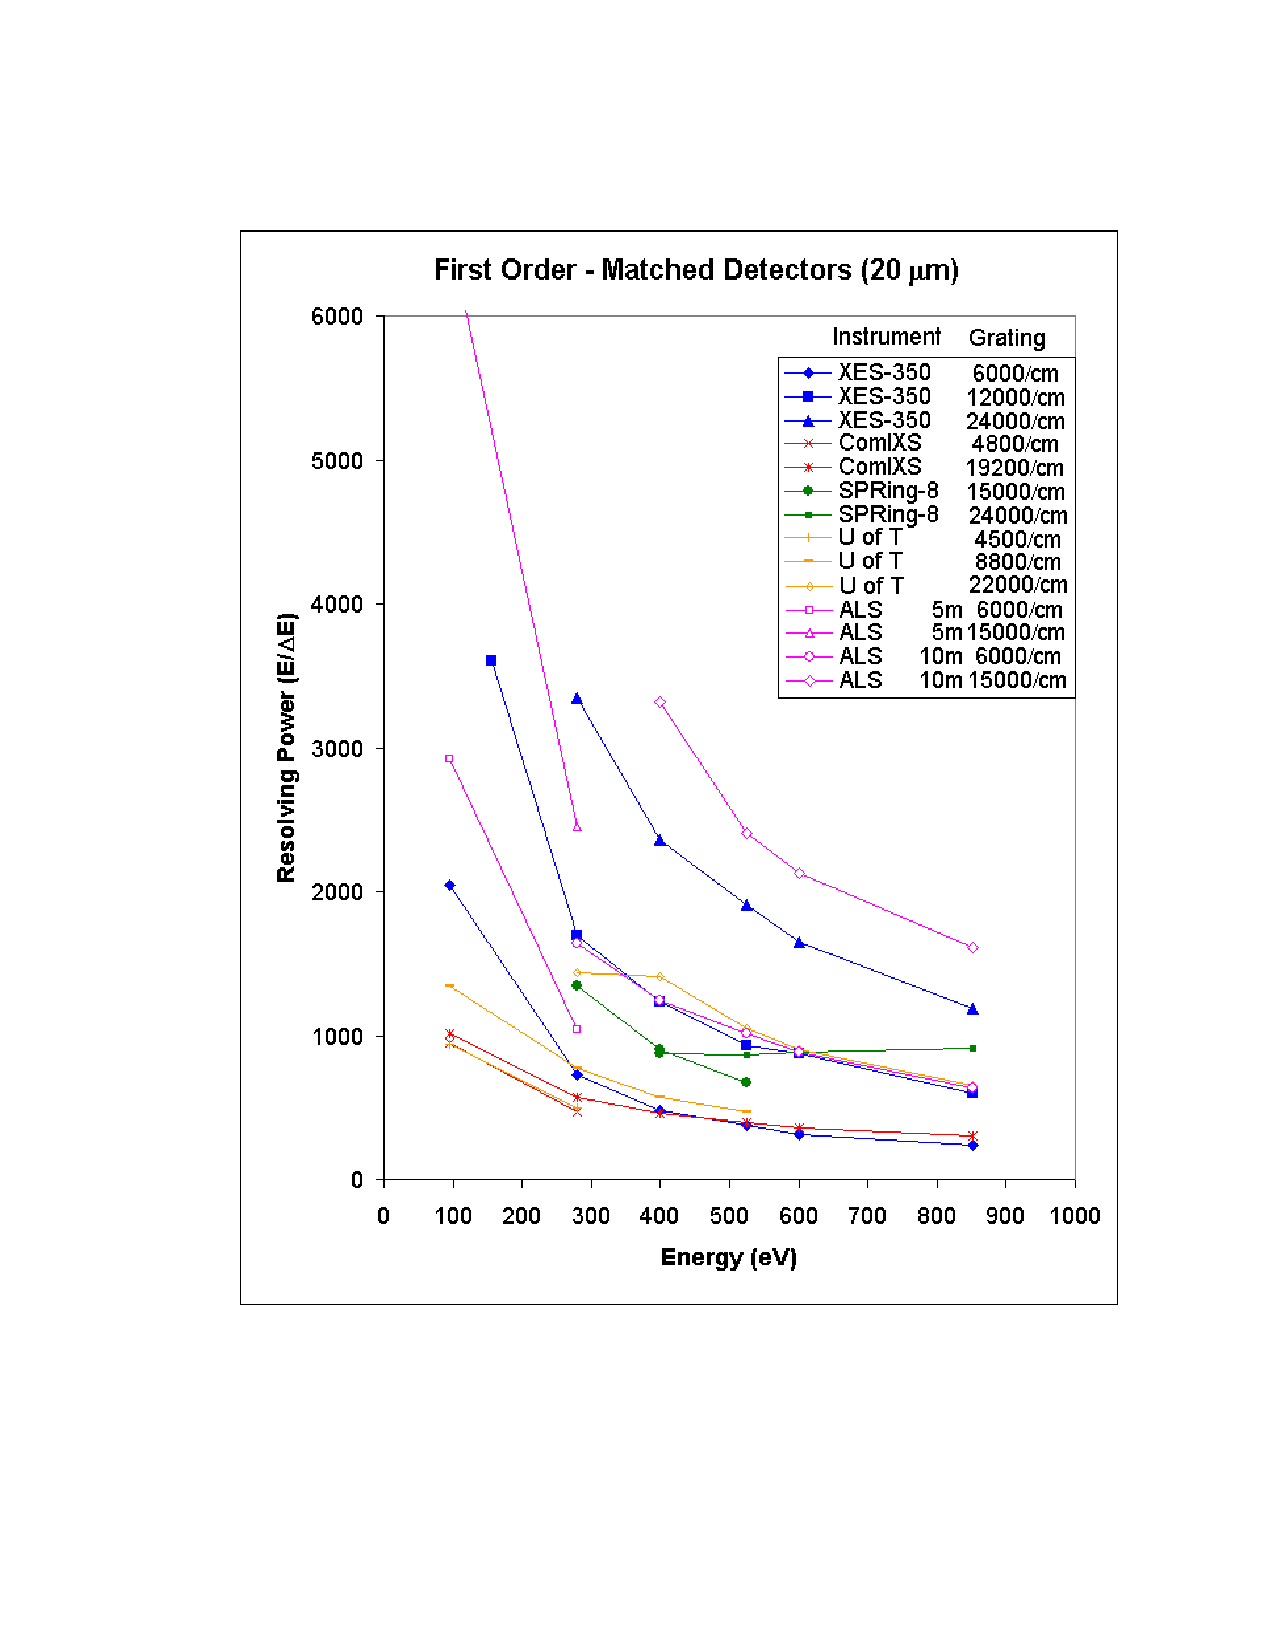
\includegraphics[width=7in]{Chapter4/4a_resolution/4a.pdf} 
   \caption{Resolving power performance comparison of existing spectrometer designs, calculated with all detectors having a 20 ?m pixel size. The legend specifies the spectrometer and grating choice (size and/or line density).  [Source: David Muir M.Sc. thesis.]}
   \label{4a}
\end{figure}

\section{Design Process}
- Iterative design process with David: jointly address factors affecting resolution

describe overlapping factors...

TABLE 4b: Factor, effect on resolution, effect on efficiency


\begin{figure}[htbp] %  figure placement: here, top, bottom, or page
   \centering
   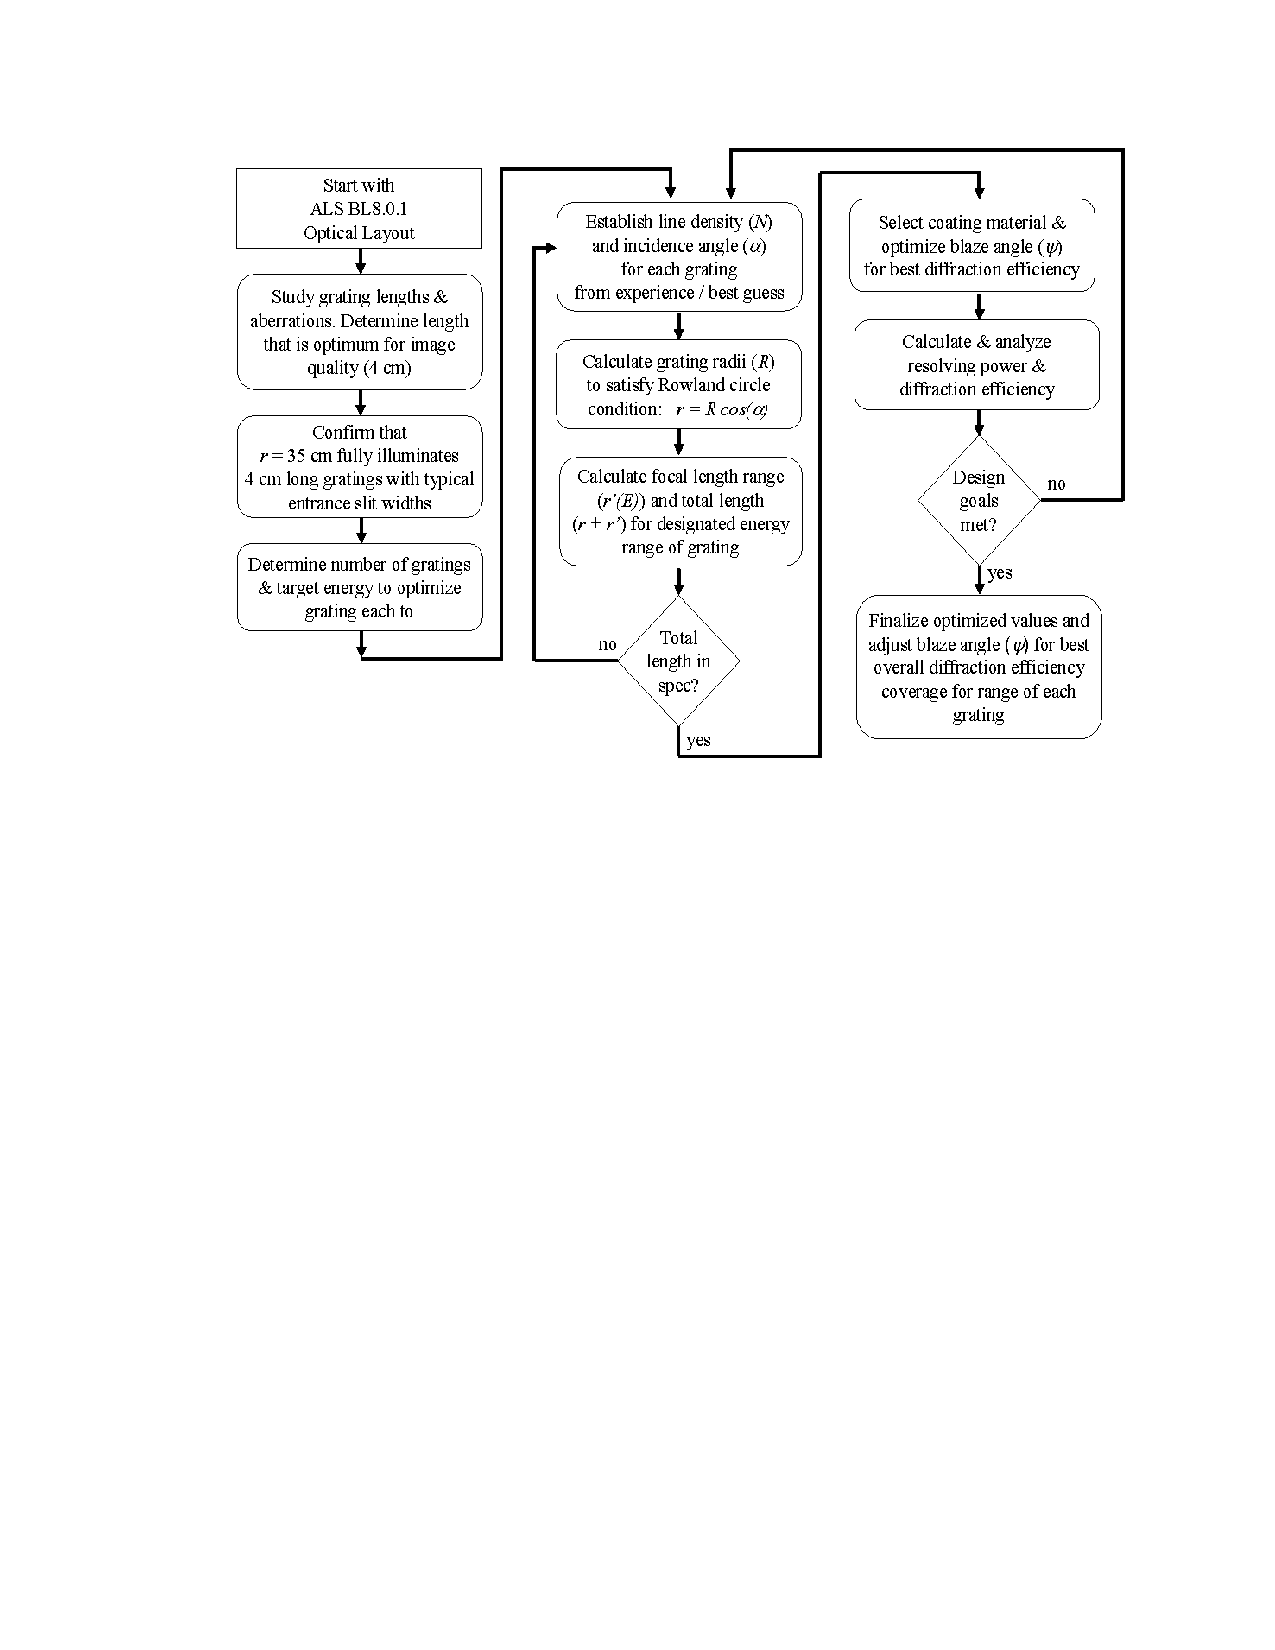
\includegraphics[scale=1]{Chapter4/4c_process/4c.pdf} 
   \caption{Approximation of the process used to design the optics of the REIXS spectrometer.  [Source: David Muir M.Sc. thesis.]}
   \label{4c}
\end{figure}

\subsection{Justification of Design choices:}
\subsubsection{Ruled vs holographic gratings}
- manufacturing errors
- holo: can't get true blaze profile... can reduce from sinusoidal using ion etching

\begin{figure}[htbp] %  figure placement: here, top, bottom, or page
   \centering
   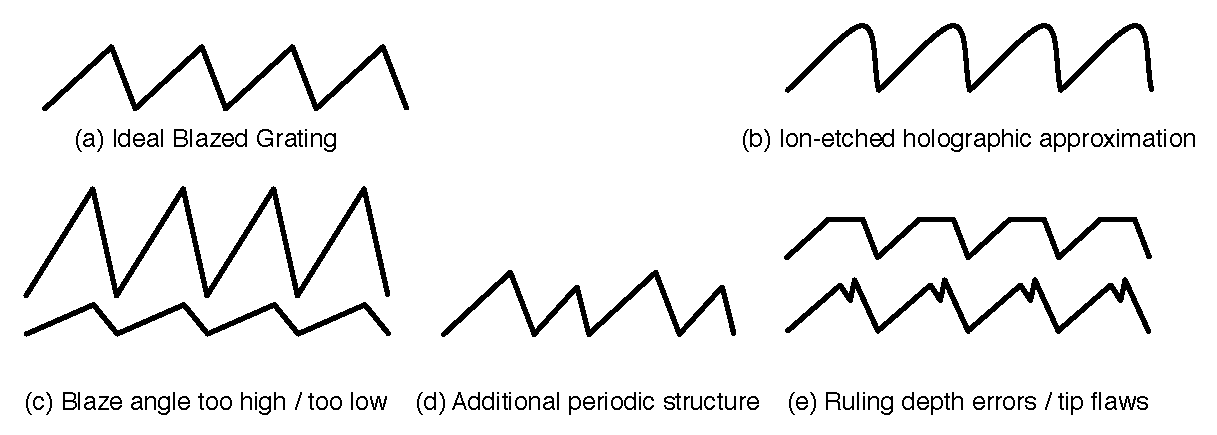
\includegraphics[scale=0.8]{Chapter4/4d_rulingFlaws/4d.pdf} 
   \caption{Common errors in the manufacture of ruled and holographic gratings.  Holographic exposure creates a sinusoidal profile; subsequent ion-etching (b) can only approximate a triangular profile.  Ruled gratings can suffer from blaze angle errors (c), or errors due to the shape and/or depth of the diamond tip (e).  If the ruling engine introduces periodic errors in the groove position, this additional structure (d) creates additional diffraction peaks (ghosts).}
   \label{4d}
\end{figure}


FIGURE 4d: common ruling errors (ideal grating; blaze angle off; ion-etched blaze; ruled blaze with large apex; ghosting)

- ruled: susceptible to "ghosting" from higher-order structure; lower upper limit on groove density; difficult and long to manufacture with precision ruling engine.  Still not true sawtooth with 90degree top corner.
\subsubsection{Rowland vs. VLS design} 
just reference david's thesis
               - VLS: flat focal curve, minimize aberrations, compact design� but lose spatial resolution for the same grating density.Examples require extremely high-res CCD detectors just to maintain average resolution.  Also: aberrations can only be fully corrected around a single energy.  Also, lose flexibility to operate in higher orders for more resolution, since the VLS optimizations depend on the order, and behave erratically outside of that. [cite: Table 3.3]  Figure 5.1
\subsubsection{blazed vs. trapezoidal/sinusoidal}
          - Not using dielectric multi-layer gratings (reason: tuned for excellence at single energy�)
\section{High-resolution (3rd order) design}
\subsection{Options for reaching extreme resolution:}
          - increase groove dens... manufacturing limit; serious drop in efficiency.
          - long detector distance (increased radius)... reduction in geometrical efficiency due to longer source-grating. [alternative: proposed design that alex reviewed: uses collecting mirror]
          - Our Novel approach: attempt usage of specially-designed blazed gratings in 3rd order. (immediately see by differentiating grating equation with respect to wavelength: effect of order on resolution)
               - Highlight: only known design in the world to do this.  Why?� Maybe we'll find out ; )
               - effect on geometric efficiency: r (source grating)
               
          DATA 4e: triple-groove dens. vs. long-distance [scaled by geometric efficiency]  vs. 3rd-order design. [note: triple-groove density would be impossible to rule]
          
\begin{figure}[htbp] %  figure placement: here, top, bottom, or page
   \centering
   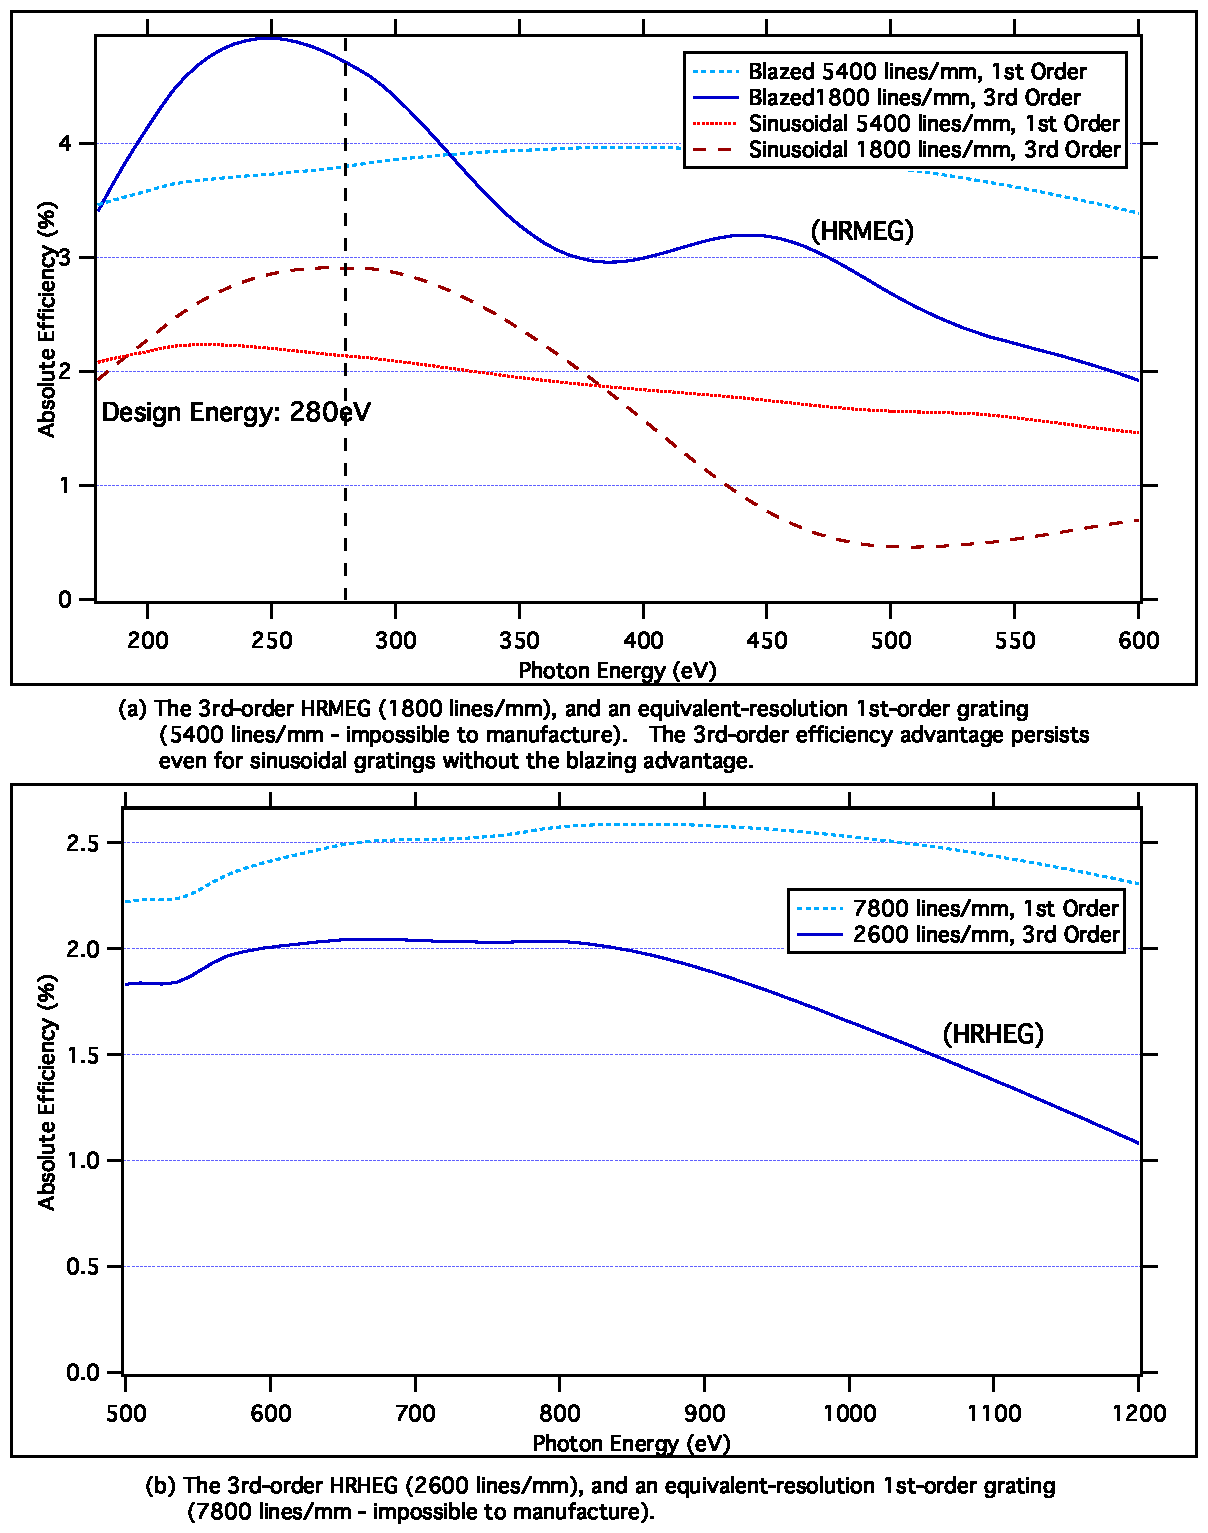
\includegraphics[scale=0.8]{Chapter4/4j_justificationFor3rdOrder/4j.pdf} 
   \caption{todo todo todo}
   \label{4e}
\end{figure}
          
          
          Alternative options to increase resolutiON
          
          
          - We were constrained at maximum machine size. Even if you could make it bigger, would it be better?
          - 
          - Increasing R:
          	- Need to maintain alpha (efficiency)
		- r and r' increase
			- First geometric efficiency hit: increase entrance arm... would need to increase grating size, but this increases cost; also limit on grating size because spherical aberrations become even more significant with grating size--> reduce focussing.   $1/r^2$
			
			- second geometric efficiency hit: increase exit distance. Only include sagittal; assume reduction in geometric efficiency due to detector catching smaller solid angle as inherent in increasing resolution.
			- spherical grating: by increasing R, also decreasing saggital focussing
			
			
			
	TODO: Why is there a peak at 87 in the incidence curve? Does it depend on material?
               
\section{Coating choices:}
     - DATA 4f: plot reflectivities over range for: Au, C, Ni, Pt, Ir, Ag, etc� [use DATA 3g]
     - Choices within regions of interest

\section{Optimization}
 simple hill-climbing [with constraints]
\section{Summary of Final Design}
	-  Key performance parameters
    	- TABLE 4g: Resolution and efficiency at emission edges of interest
	
	- DATA 4h: efficiency plots for each grating
	
\begin{figure}[htbp] %  figure placement: here, top, bottom, or page
   \centering
   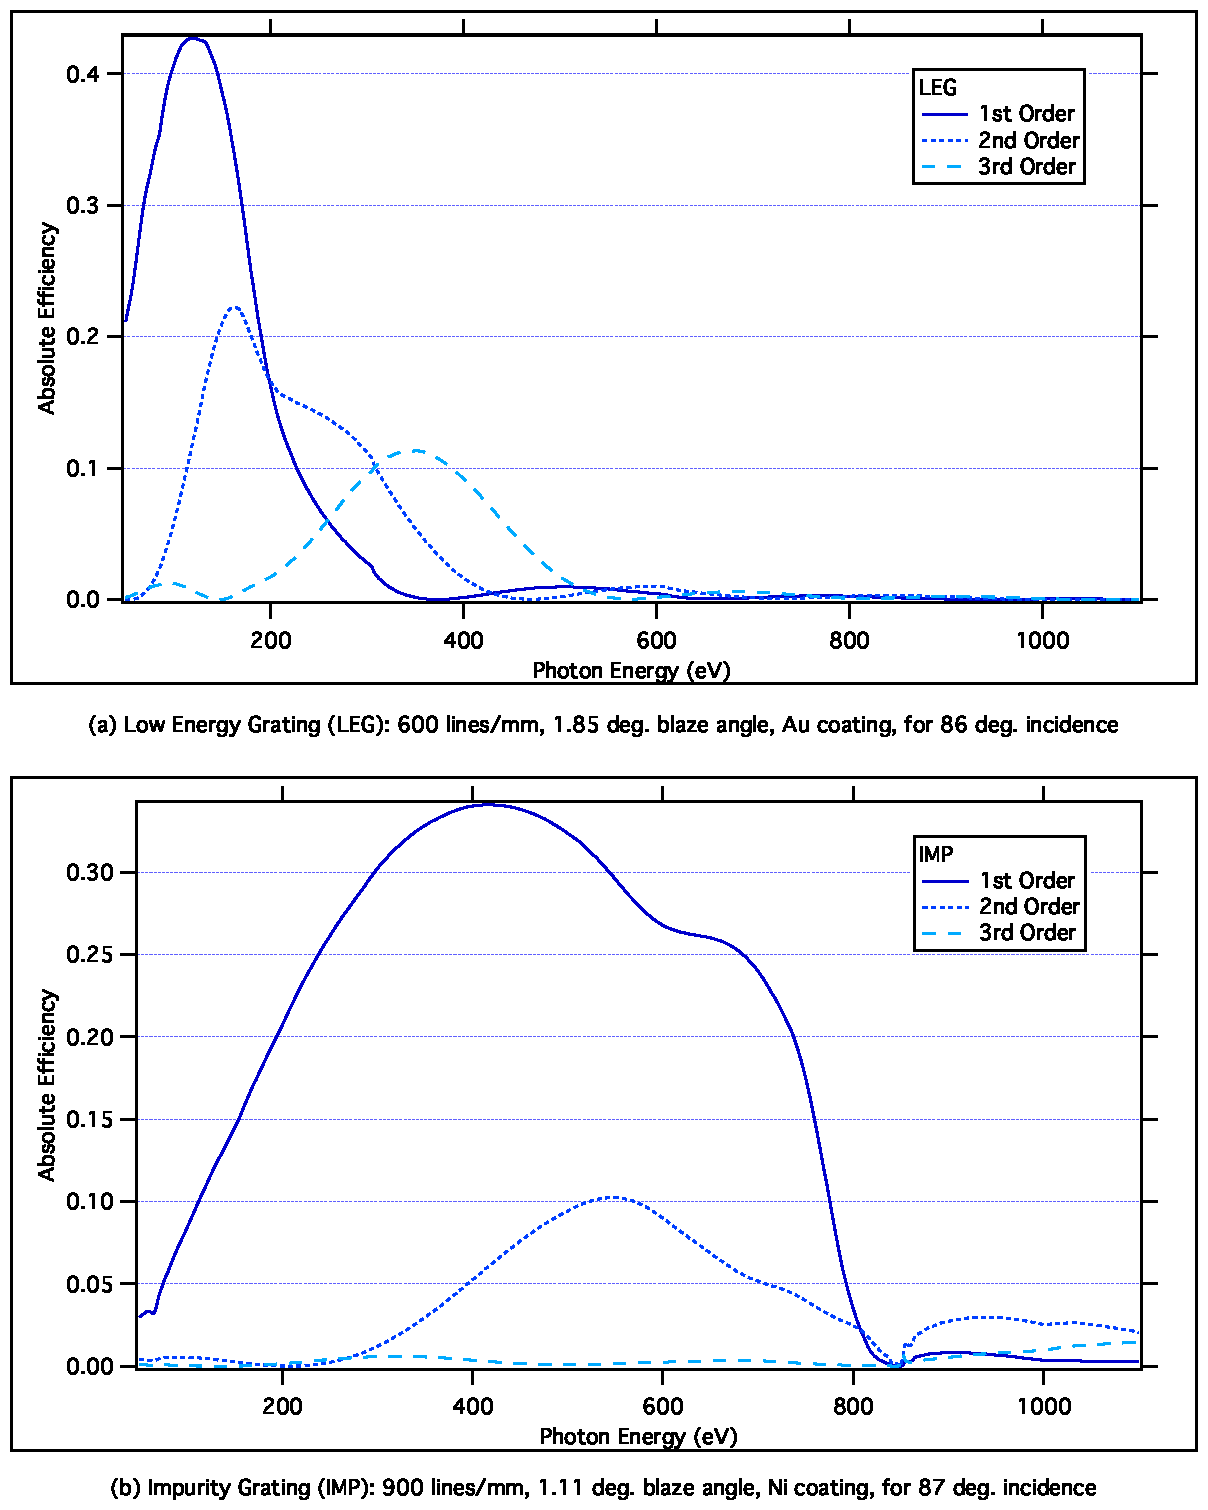
\includegraphics[scale=0.8]{Chapter4/4h_gratings/LEG_IMP.pdf} 
   \caption{Theoretical diffraction efficiency for the Low Energy Grating and Impurity Grating, as designed}
   \label{4h-1}
\end{figure}

\begin{figure}[htbp] %  figure placement: here, top, bottom, or page
   \centering
   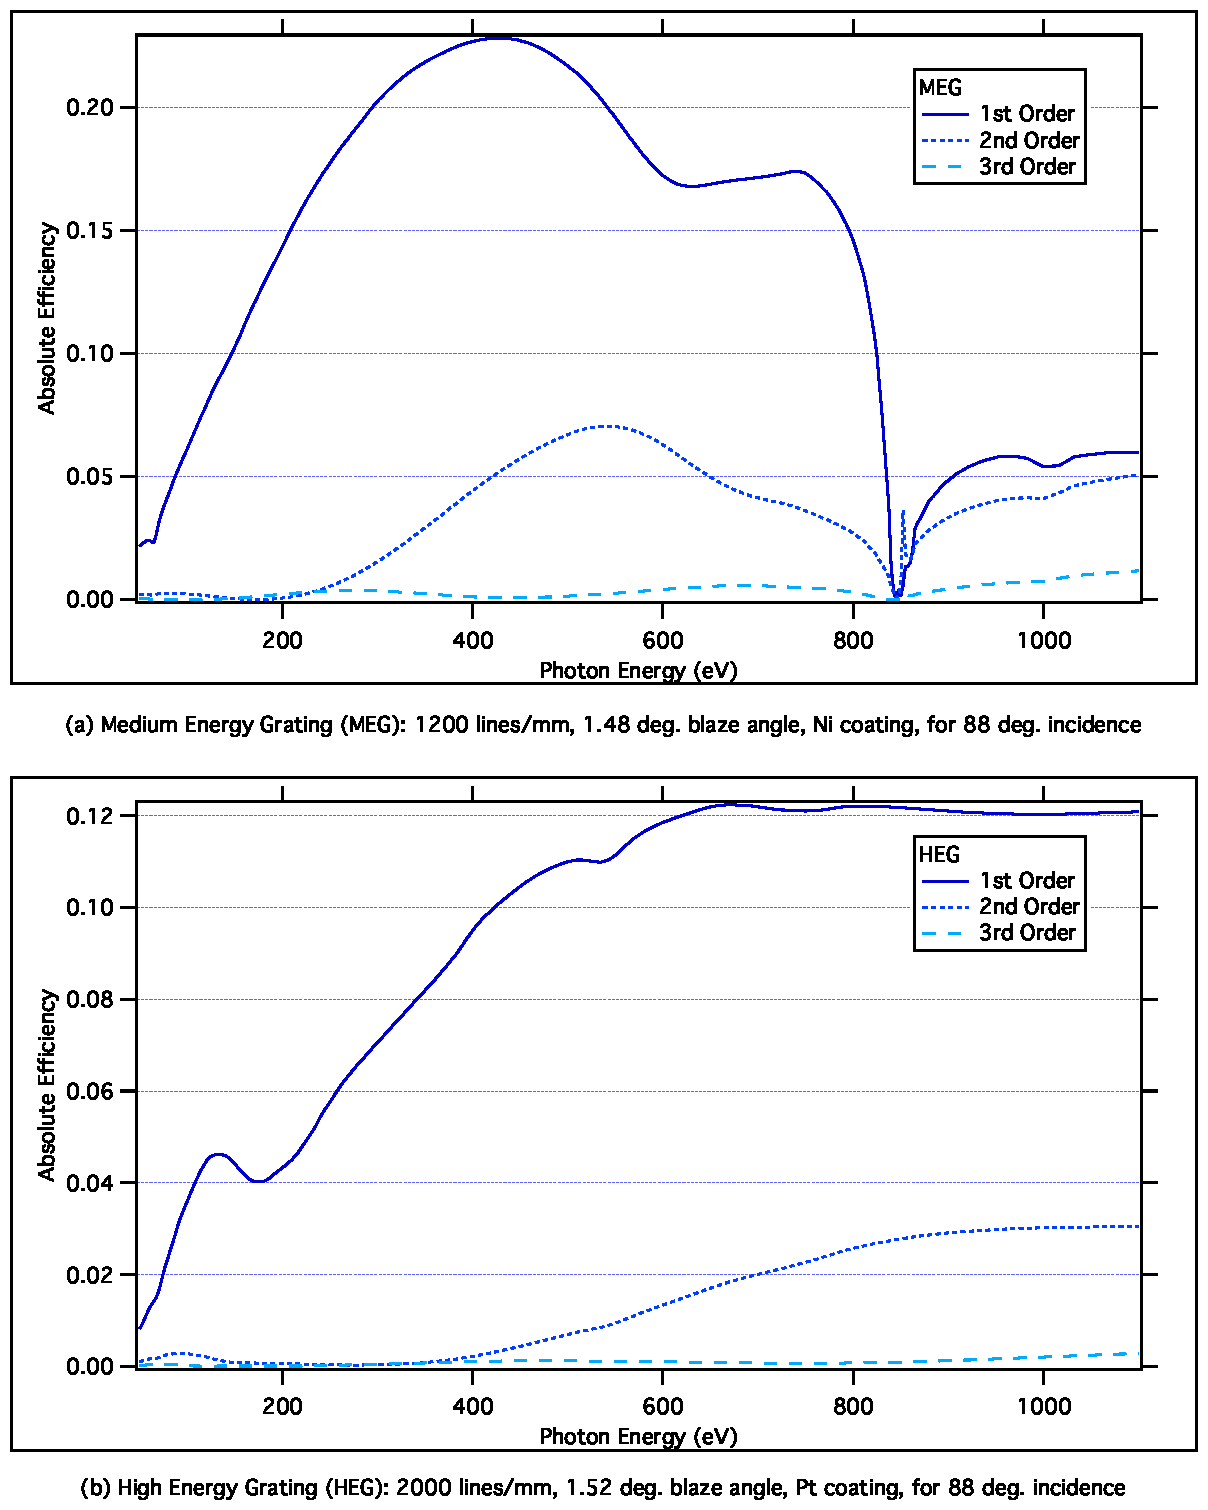
\includegraphics[scale=0.8]{Chapter4/4h_gratings/MEG_HEG.pdf} 
   \caption{Theoretical diffraction efficiency for the Medium Energy and High Energy Gratings, as designed}
   \label{4h-2}
\end{figure}

\begin{figure}[htbp] %  figure placement: here, top, bottom, or page
   \centering
   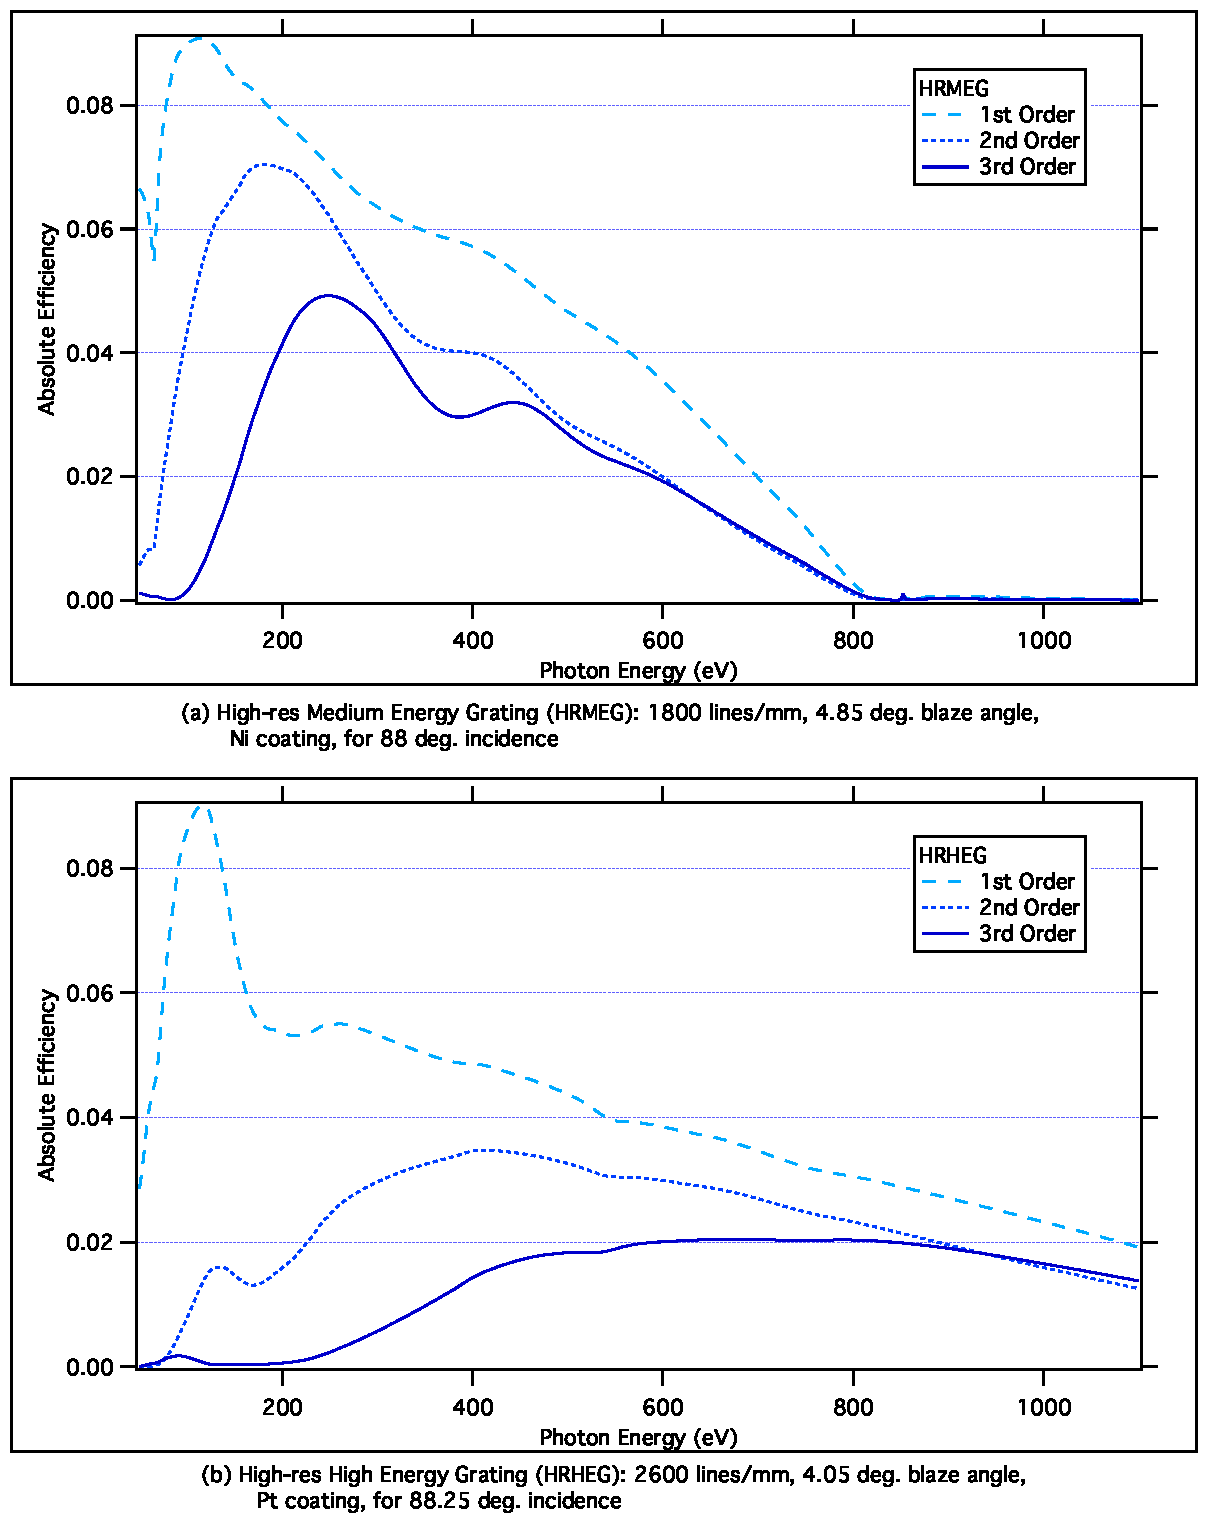
\includegraphics[scale=0.8]{Chapter4/4h_gratings/HRMEG_HRHEG.pdf} 
   \caption{Theoretical diffraction efficiency for the High Resolution Gratings, optimized to be used in 3rd order.}
   \label{4h-3}
\end{figure}


Note: effect of blazing: profound at low energies and low groove densities.  Less pronounced "humps" at higher energies and groove densities.
EXPLORE: Optimize an LEG for 800eV. Still humps? Effect due to groove dens, energy, or incidence? [LEG is low on all of those]

